\chapter{Results and Analysis}
\label{ch:results}

\section{Quantitative Overview}
\label{sec:quant}

Table~\ref{tab:ranking} ranks jurisdictions by unweighted composite score $S_c$ (Equation~\eqref{eq:composite}). Table~\ref{tab:themeavg} summarizes global theme means and ranges. The full seven-theme matrix appears in Table~\ref{tab:country-scores}. Visual summaries generated from the open dataset published with the Streamlit dashboard\footnote{\repoLink{}} are shown in Figures~\ref{fig:ranking}--\ref{fig:gap}.

\begin{table}[htbp]
\centering
\caption{Jurisdictions ranked by composite compliance score $S_c$}
\label{tab:ranking}
\renewcommand{\arraystretch}{1.15}
\begin{tabular}{@{}lllc!{\color{black!25}\vrule width 0.8pt}r@{}}
\toprule
\textbf{Country} & \textbf{Region} & \textbf{Maturity} & \textbf{$S_c$} &
\multicolumn{1}{c}{\textbf{\footnotesize Devices}\textsuperscript{\dag}} \\
\midrule
European Union & Europe & Advanced & 9.14 & 600 \\
Germany & Europe & Advanced & 8.71 & 180 \\
United States & North America & Advanced & 7.57 & 950 \\
United Kingdom & Europe & Advanced & 7.14 & 200 \\
Canada & North America & Advanced & 7.14 & 120 \\
Japan & Asia & Advanced & 7.00 & 150 \\
Singapore & Asia & Advanced & 6.86 & 60 \\
Switzerland & Europe & Advanced & 6.86 & 90 \\
China & Asia & Advanced & 6.71 & 300 \\
Australia & Oceania & Moderate & 6.57 & 80 \\
South Korea & Asia & Advanced & 6.57 & 200 \\
Israel & Middle East & Advanced & 6.29 & 100 \\
Brazil & South America & Developing & 5.29 & 40 \\
UAE & Middle East & Emerging & 4.57 & 35 \\
Saudi Arabia & Middle East & Emerging & 4.43 & 25 \\
India & Asia & Developing & 4.29 & 30 \\
Thailand & Asia & Developing & 3.86 & 15 \\
South Africa & Africa & Emerging & 3.57 & 10 \\
Kenya & Africa & Early & 2.71 & 3 \\
Nigeria & Africa & Early & 2.57 & 5 \\
\bottomrule
\end{tabular}

\vspace{0.35em}
{\footnotesize\textsuperscript{\dag}\textit{Devices} = reported AI/ML device authorizations (throughput metric; not part of $S_c$ and not cross-border comparable---see Section~\ref{sec:devicecounts}).}
\end{table}

\begin{figure}[htbp]
\centering
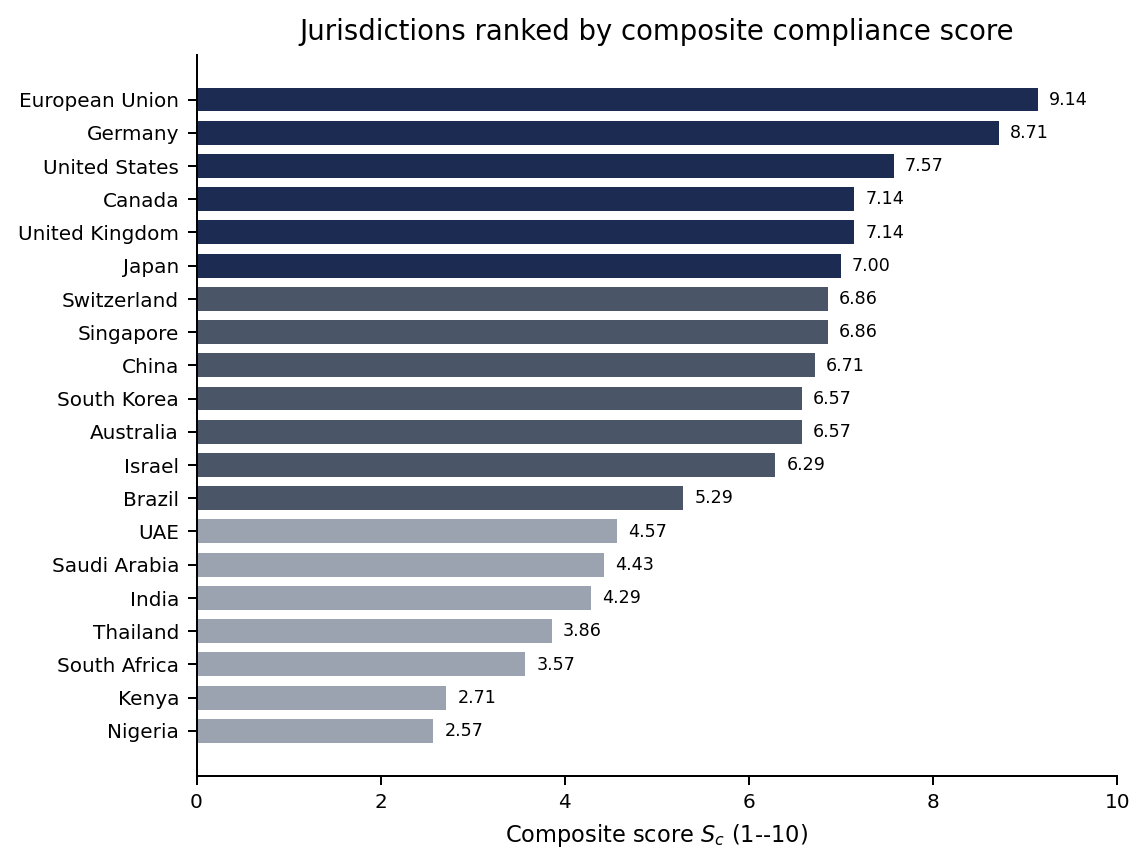
\includegraphics[width=0.70\textwidth]{figures/fig_composite_ranking.png}
\caption{Composite score ranking across 20 jurisdictions (source: curated dataset).}
\label{fig:ranking}
\end{figure}

\begin{table}[htbp]
\centering
\caption{Global theme score statistics across 20 jurisdictions}
\label{tab:themeavg}
\begin{tabular}{@{}lccc@{}}
\toprule
\textbf{Theme} & \textbf{Mean} & \textbf{Min} & \textbf{Max} \\
\midrule
Data privacy & 6.70 & 4 & 10 \\
Clinical validation & 6.20 & 2 & 9 \\
Approval process & 6.30 & 3 & 9 \\
Transparency & 5.60 & 2 & 9 \\
Ethics & 5.95 & 3 & 10 \\
Post-market & 5.75 & 2 & 9 \\
Liability & 4.75 & 2 & 8 \\
\bottomrule
\end{tabular}
\end{table}

\begin{figure}[htbp]
\centering
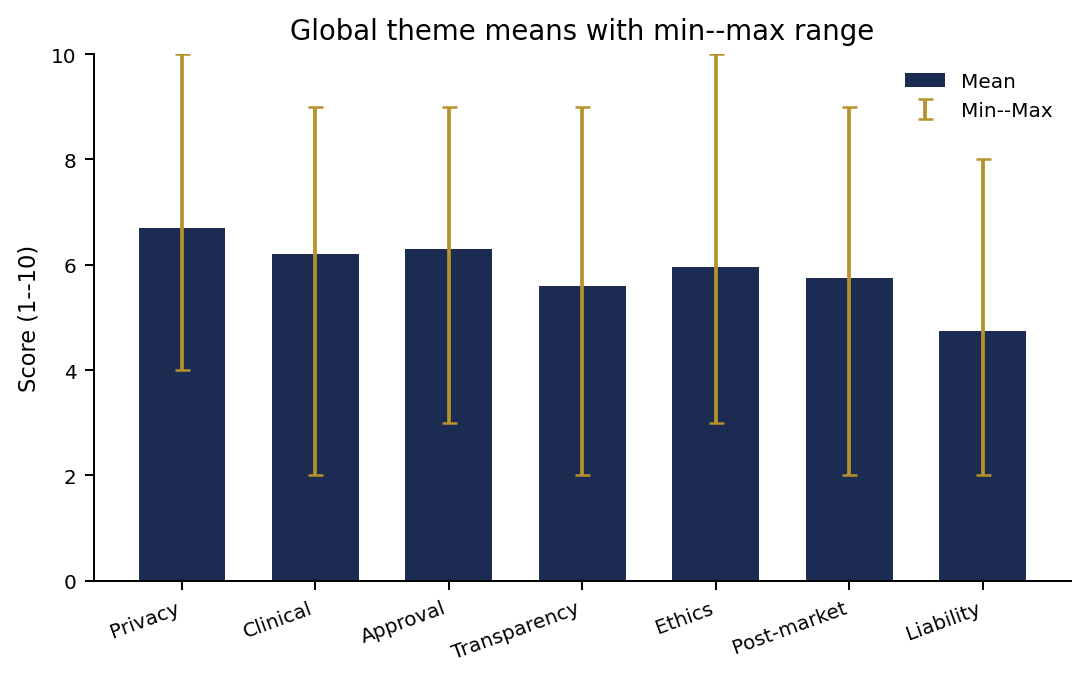
\includegraphics[width=0.68\textwidth]{figures/fig_theme_means.png}
\caption{Global theme means with min--max ranges.}
\label{fig:theme-means}
\end{figure}

\begin{table}[htbp]
\centering
\caption{Complete seven-theme compliance scores for all 20 jurisdictions}
\label{tab:country-scores}
\scriptsize
\begin{tabular}{@{}l ccccccc c@{}}
\toprule
\textbf{Country} & \textbf{Priv.} & \textbf{Clin.} & \textbf{Appr.} & \textbf{Trans.} & \textbf{Eth.} & \textbf{Post} & \textbf{Liab.} & $\boldsymbol{S_c}$ \\
\midrule
European Union & 10 & 9 & 9 & 9 & 10 & 9 & 8 & 9.14 \\
Germany & 10 & 9 & 9 & 8 & 9 & 9 & 7 & 8.71 \\
United States & 8 & 9 & 9 & 6 & 6 & 8 & 7 & 7.57 \\
United Kingdom & 8 & 8 & 7 & 7 & 7 & 7 & 6 & 7.14 \\
Canada & 7 & 8 & 8 & 7 & 7 & 7 & 6 & 7.14 \\
Japan & 7 & 8 & 8 & 6 & 7 & 8 & 5 & 7.00 \\
Singapore & 7 & 7 & 7 & 8 & 8 & 6 & 5 & 6.86 \\
Switzerland & 8 & 8 & 8 & 6 & 6 & 7 & 5 & 6.86 \\
China & 7 & 7 & 7 & 7 & 6 & 7 & 6 & 6.71 \\
Australia & 7 & 7 & 7 & 6 & 7 & 7 & 5 & 6.57 \\
South Korea & 7 & 7 & 8 & 6 & 6 & 7 & 5 & 6.57 \\
Israel & 6 & 8 & 7 & 6 & 6 & 6 & 5 & 6.29 \\
Brazil & 7 & 5 & 5 & 5 & 5 & 5 & 5 & 5.29 \\
UAE & 5 & 5 & 5 & 5 & 5 & 4 & 3 & 4.57 \\
Saudi Arabia & 5 & 4 & 5 & 5 & 5 & 4 & 3 & 4.43 \\
India & 5 & 4 & 4 & 4 & 5 & 4 & 4 & 4.29 \\
Thailand & 5 & 4 & 4 & 4 & 4 & 3 & 3 & 3.86 \\
South Africa & 6 & 3 & 3 & 3 & 4 & 3 & 3 & 3.57 \\
Kenya & 5 & 2 & 3 & 2 & 3 & 2 & 2 & 2.71 \\
Nigeria & 4 & 2 & 3 & 2 & 3 & 2 & 2 & 2.57 \\
\bottomrule
\end{tabular}
\end{table}


\begin{table}[htbp]
\centering
\caption{Geographic coverage of the compliance dataset (20 jurisdictions)}
\label{tab:coverage}
\begin{tabularx}{\textwidth}{@{}l X@{}}
\toprule
\textbf{Region} & \textbf{Jurisdictions} \\
\midrule
Africa & South Africa, Nigeria, Kenya \\
Asia & China, India, Japan, South Korea, Singapore, Thailand \\
Europe & European Union, United Kingdom, Switzerland, Germany \\
Middle East & Saudi Arabia, Israel, UAE \\
North America & United States, Canada \\
Oceania & Australia \\
South America & Brazil \\
\bottomrule
\end{tabularx}
\end{table}

\begin{table}[htbp]
\centering
\caption{Count of jurisdictions by regulatory maturity label}
\label{tab:maturity-counts}
\begin{tabular}{@{}lc@{}}
\toprule
\textbf{Maturity} & \textbf{Count} \\
\midrule
Advanced & 11 \\
Moderate & 1 \\
Developing & 3 \\
Emerging & 3 \\
Early & 2 \\
\bottomrule
\end{tabular}
\end{table}

\begin{table}[htbp]
\centering
\caption{Regional mean theme scores (1--10) derived from the curated dataset}
\label{tab:regional-means}
\begin{tabular}{@{}lccccccc@{}}
\toprule
\textbf{Region} & \textbf{Priv.} & \textbf{Clin.} & \textbf{Appr.} & \textbf{Trans.} & \textbf{Eth.} & \textbf{Post} & \textbf{Liab.} \\
\midrule
Africa & 5.0 & 2.3 & 3.0 & 2.3 & 3.3 & 2.3 & 2.3 \\
Asia & 6.3 & 6.2 & 6.3 & 5.8 & 6.0 & 5.8 & 4.7 \\
Europe & 9.0 & 8.5 & 8.2 & 7.5 & 8.0 & 8.0 & 6.5 \\
Middle East & 5.3 & 5.7 & 5.7 & 5.3 & 5.3 & 4.7 & 3.7 \\
North America & 7.5 & 8.5 & 8.5 & 6.5 & 6.5 & 7.5 & 6.5 \\
Oceania & 7.0 & 7.0 & 7.0 & 6.0 & 7.0 & 7.0 & 5.0 \\
South America & 7.0 & 5.0 & 5.0 & 5.0 & 5.0 & 5.0 & 5.0 \\
\bottomrule
\end{tabular}
\end{table}


\begin{figure}[htbp]
\centering
\begin{minipage}[t]{0.48\textwidth}
\centering
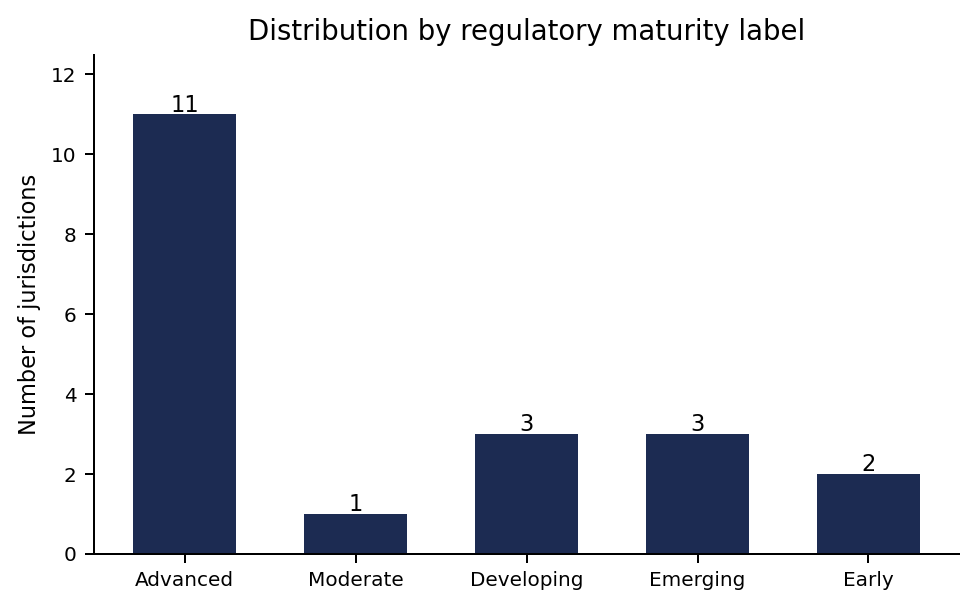
\includegraphics[width=\linewidth]{figures/fig_maturity_distribution.png}
\caption{Distribution of jurisdictions by maturity label.}
\label{fig:maturity}
\end{minipage}\hfill
\begin{minipage}[t]{0.48\textwidth}
\centering
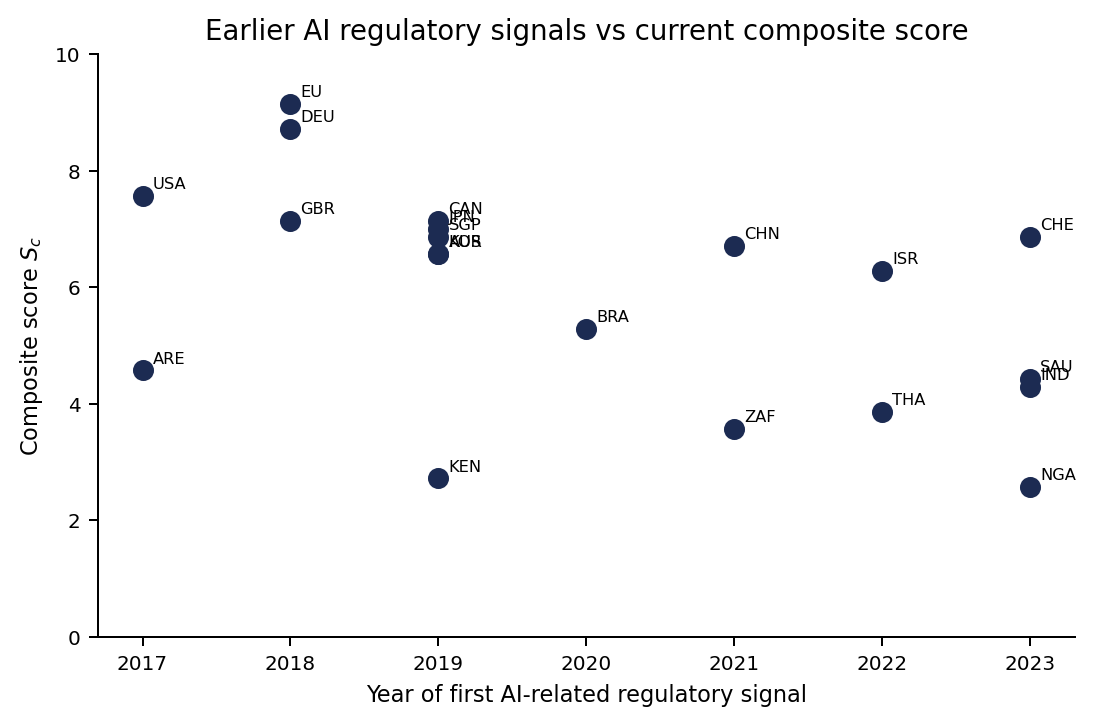
\includegraphics[width=\linewidth]{figures/fig_year_vs_score.png}
\caption{Year of first AI regulatory signal vs composite score.}
\label{fig:yearscore}
\end{minipage}
\end{figure}

\begin{figure}[htbp]
\centering
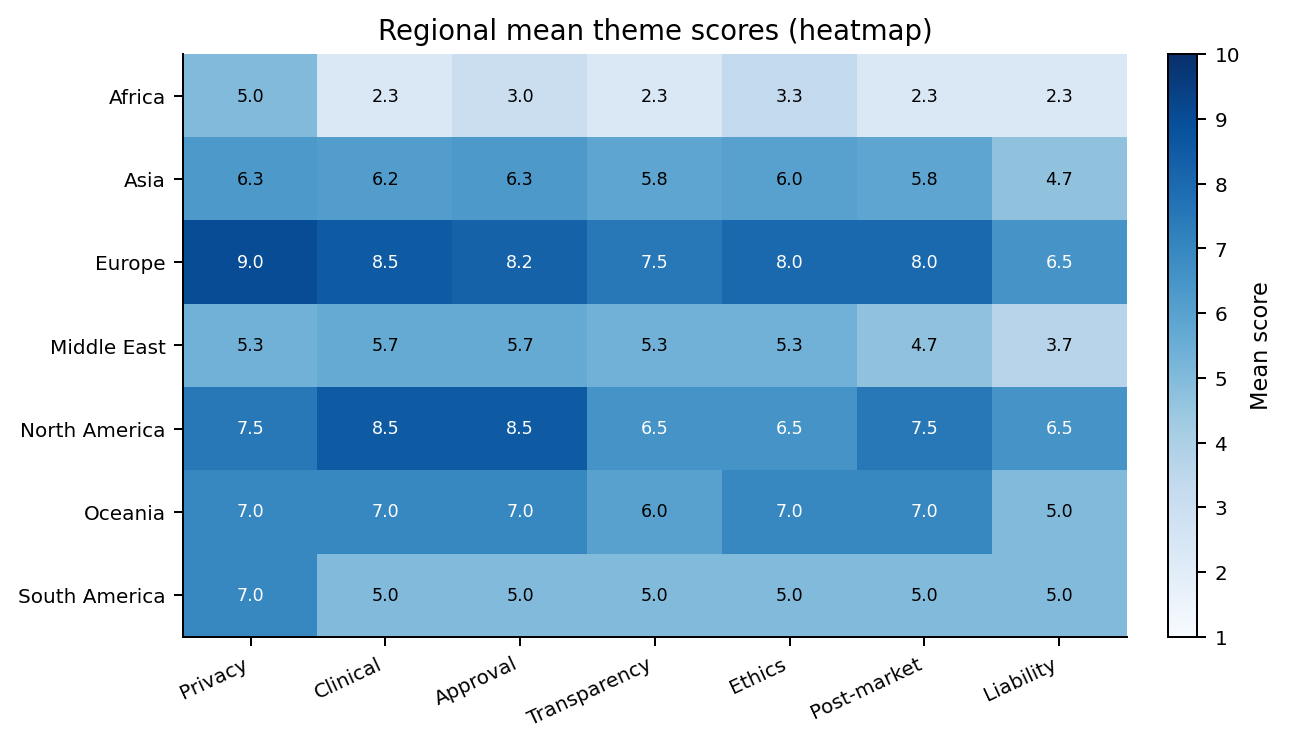
\includegraphics[width=0.78\textwidth]{figures/fig_regional_heatmap.png}
\caption{Regional mean theme scores visualized as a heatmap.}
\label{fig:heatmap}
\end{figure}

\begin{figure}[htbp]
\centering
\begin{minipage}[t]{0.46\textwidth}
\centering
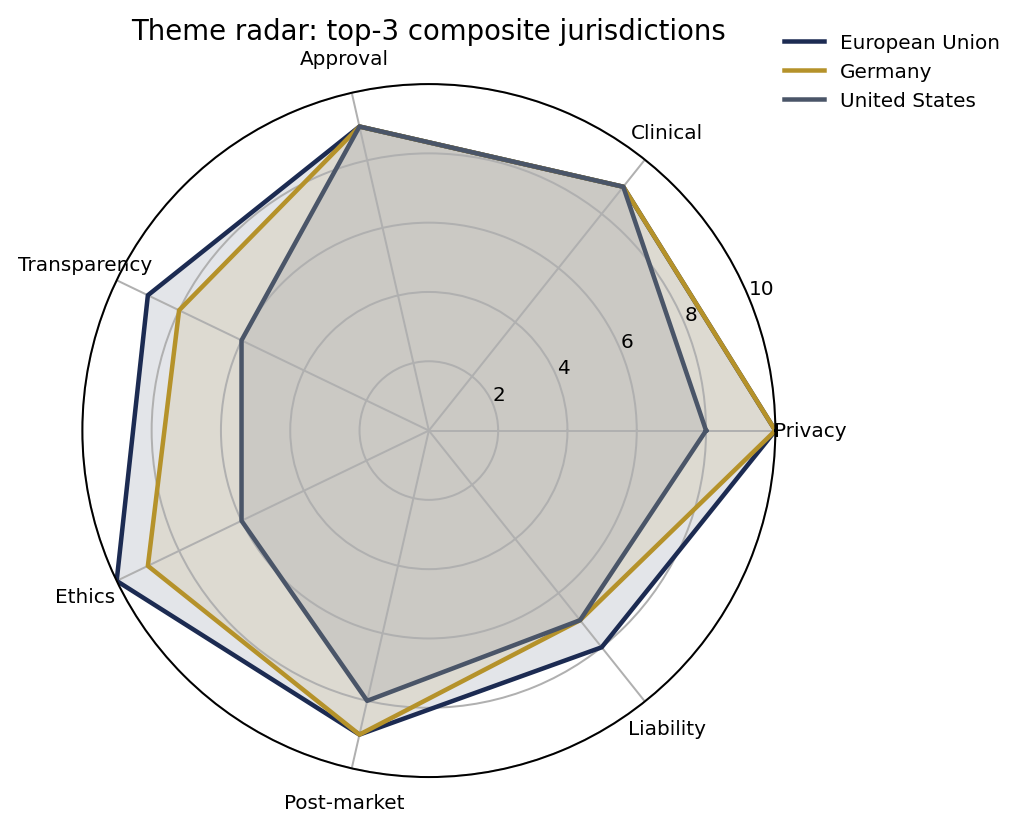
\includegraphics[width=\linewidth]{figures/fig_radar_top3.png}
\caption{Radar comparison of the top-3 composite jurisdictions.}
\label{fig:radar}
\end{minipage}\hfill
\begin{minipage}[t]{0.50\textwidth}
\centering
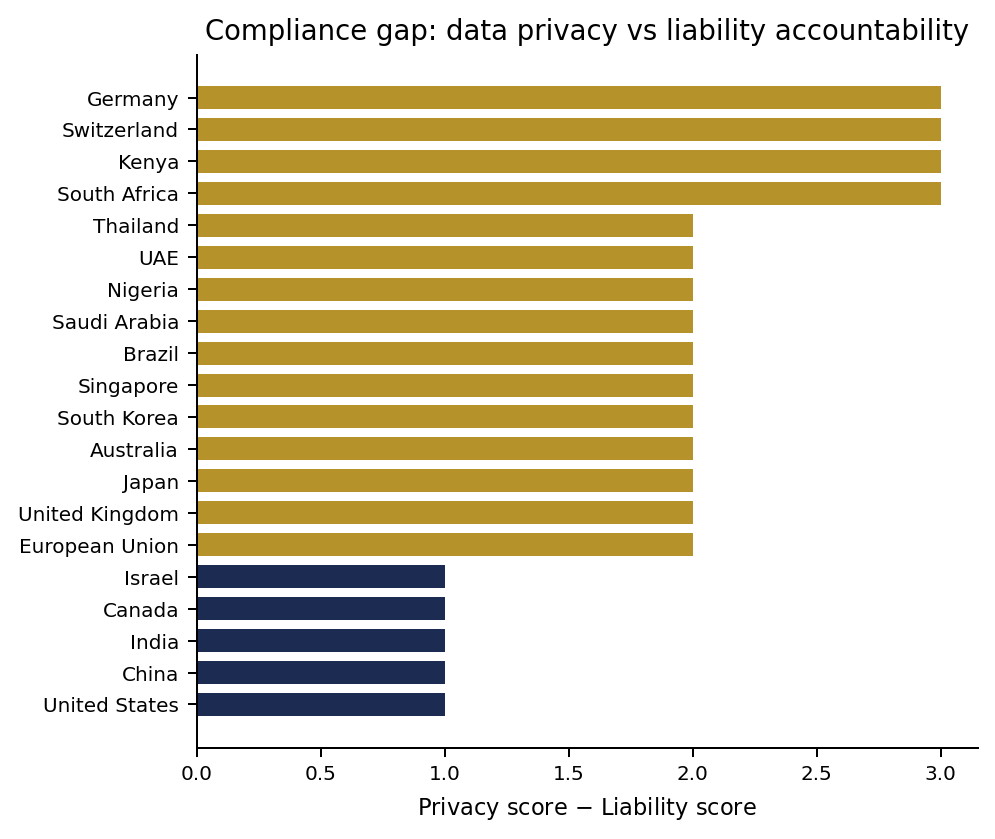
\includegraphics[width=\linewidth]{figures/fig_privacy_liability_gap.png}
\caption{Privacy minus liability theme gap (gold: gap $\geq 2$).}
\label{fig:gap}
\end{minipage}
\end{figure}

\begin{figure}[htbp]
\centering
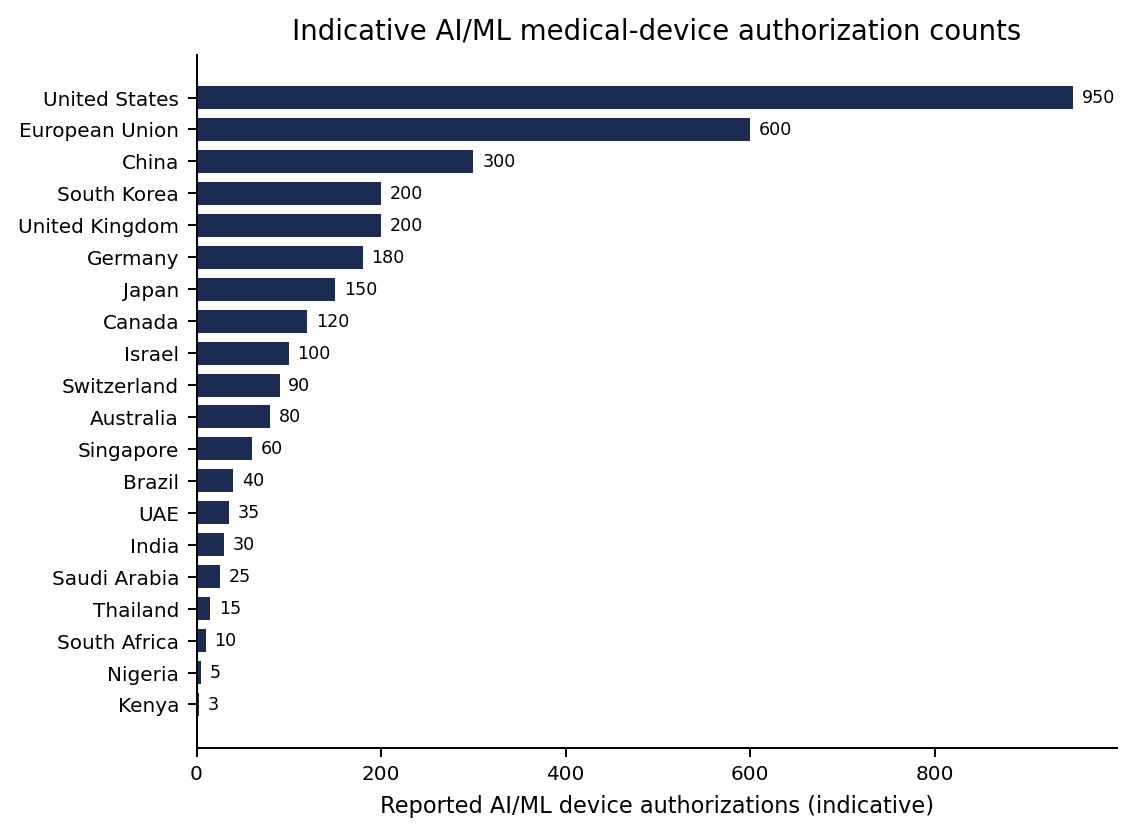
\includegraphics[width=0.70\textwidth]{figures/fig_device_approvals.png}
\caption{Indicative AI/ML medical-device authorization counts (not commensurate across agencies).}
\label{fig:devices}
\end{figure}

\begin{figure}[htbp]
\centering
\begin{minipage}[t]{0.48\textwidth}
\centering
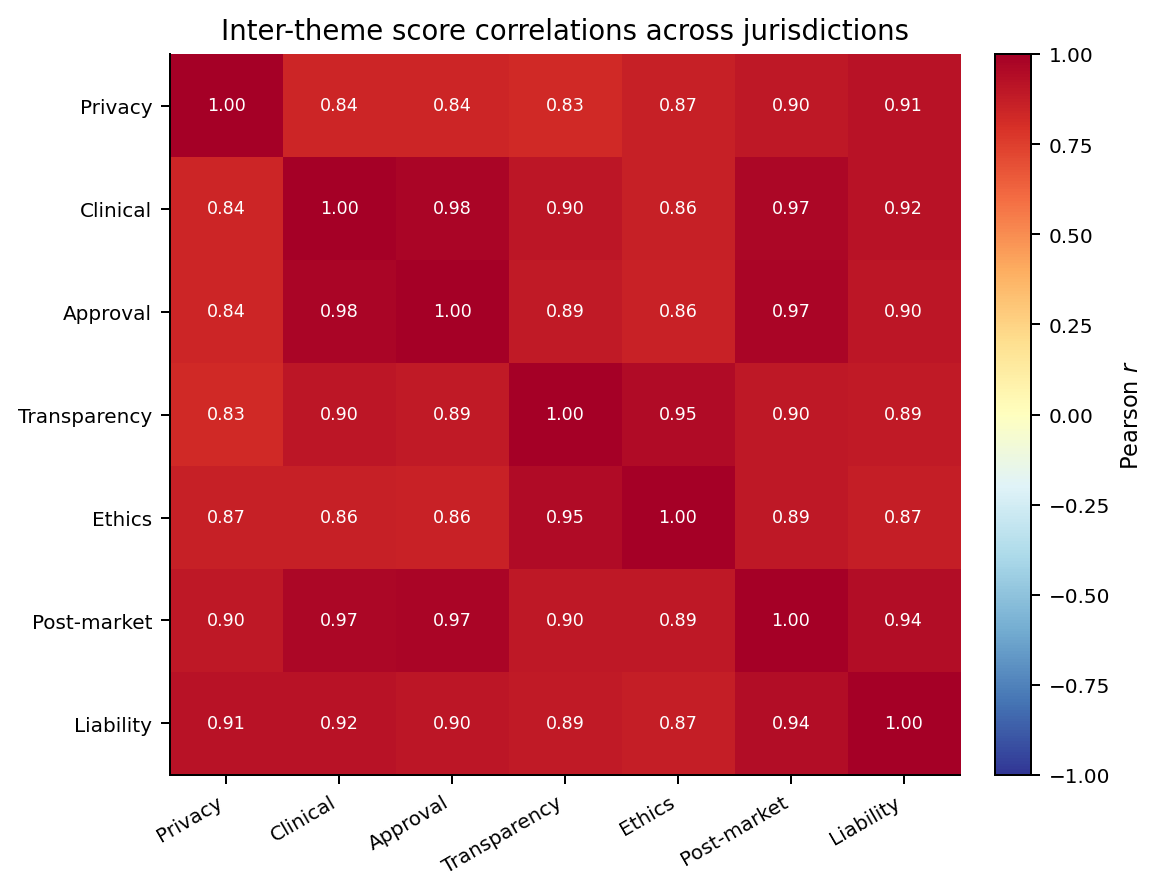
\includegraphics[width=\linewidth]{figures/fig_theme_correlation.png}
\caption{Inter-theme Pearson correlations across jurisdictions.}
\label{fig:theme-corr}
\end{minipage}\hfill
\begin{minipage}[t]{0.48\textwidth}
\centering
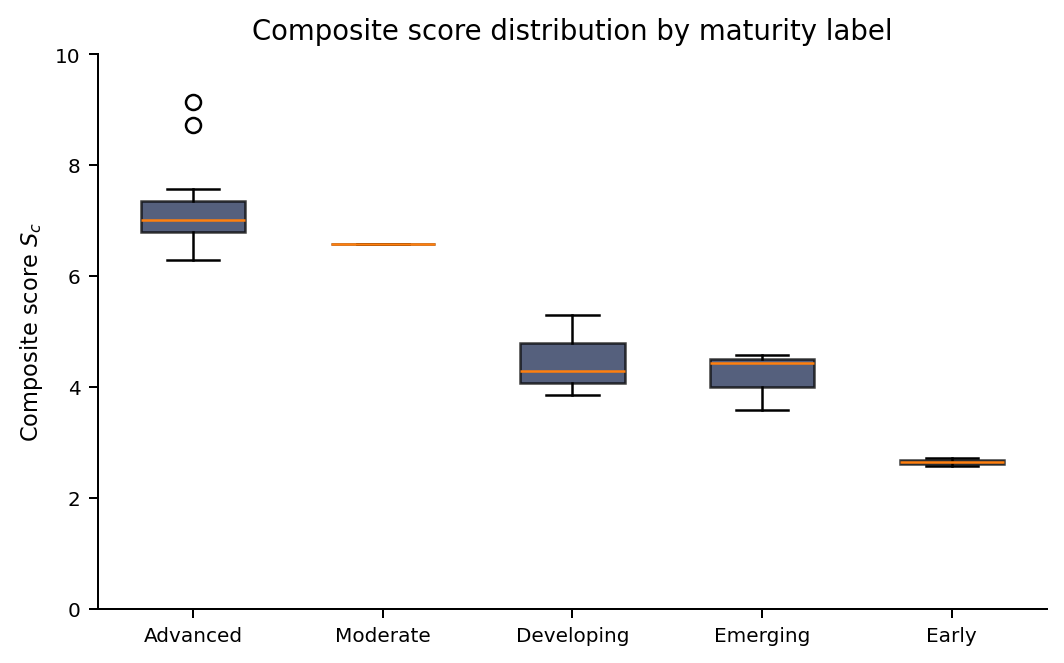
\includegraphics[width=\linewidth]{figures/fig_box_maturity.png}
\caption{Composite score distribution by maturity label.}
\label{fig:box-maturity}
\end{minipage}
\end{figure}

\begin{figure}[htbp]
\centering
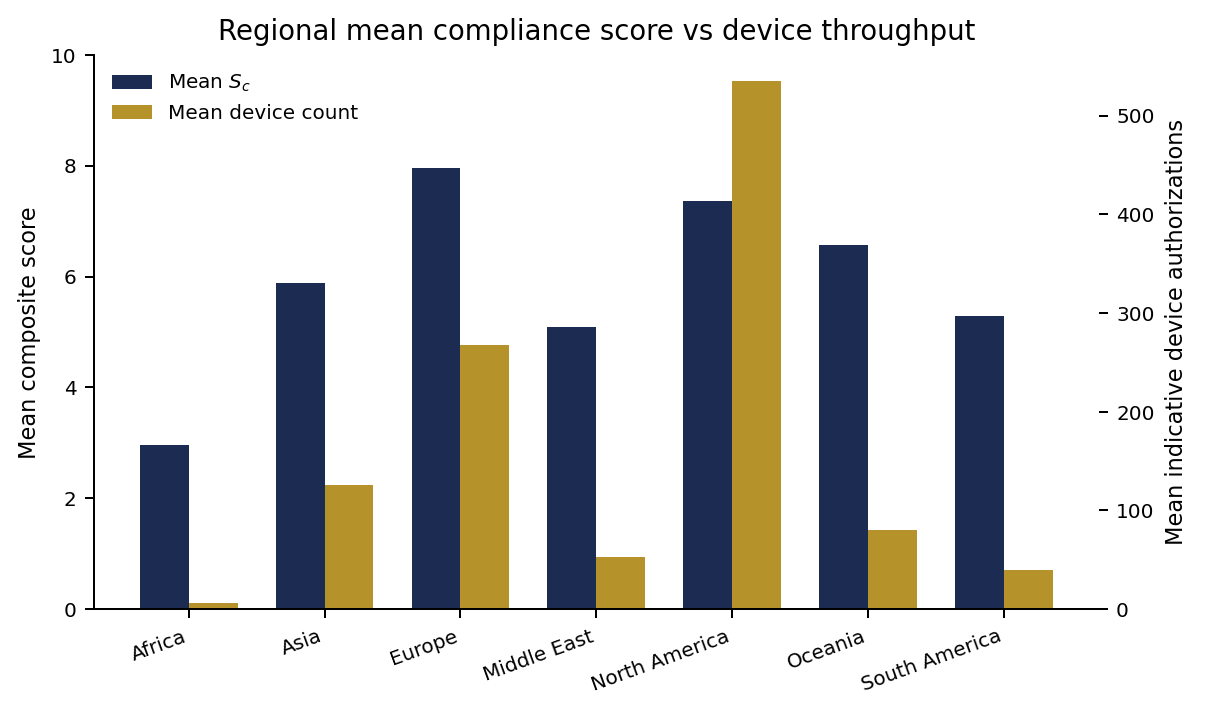
\includegraphics[width=0.78\textwidth]{figures/fig_region_score_vs_devices.png}
\caption{Regional mean compliance score versus mean indicative device authorizations.}
\label{fig:region-devices}
\end{figure}

\section{Interpretation of Global Patterns}
\label{sec:patterns}

Across the curated set, \textbf{data privacy} and \textbf{approval process} themes tend to score relatively high on average, reflecting the post-GDPR legislative wave and the near-universal presence of medical-device frameworks. \textbf{Liability} and, in several emerging jurisdictions, \textbf{post-market surveillance} and \textbf{transparency} lag---indicating that lifecycle governance and accountability remain frontier issues even where market-entry pathways exist. Figure~\ref{fig:gap} makes this asymmetry explicit: many jurisdictions score privacy substantially higher than liability.

Europe (including the EU aggregate and Germany) leads on composite scores, consistent with the layered GDPR + MDR + AI Act regime~\cite{euaiact2024}. The United States leads on reported device throughput while showing comparatively moderate transparency/ethics scores, matching the literature's characterization of an innovation-forward, less horizontally mandated AI ethics posture~\cite{fda2021,wu2021}. East Asian advanced jurisdictions combine substantial approval activity with evolving privacy and algorithm rules. African and some Middle Eastern entries illustrate data-protection progress preceding deep AI-SaMD capacity.


\section{Regional Qualitative Analysis}
\label{sec:regional}

\subsection{North America}
The USA--Canada pair demonstrates advanced agency science and GMLP leadership~\cite{gmlp2021}, with U.S.\ HIPAA sectoral privacy contrasting Canada's more comprehensive federal privacy trajectory. Fragmentation (U.S.\ state privacy; Canadian legislative timing) remains a practical compliance challenge for multi-province/multi-state deployments.

\subsection{Europe}
The EU AI Act is a watershed for binding high-risk obligations~\cite{euaiact2024}. Germany's strong scores reflect both EU baselines and national digital-health instrumentation. The UK's post-Brexit pro-innovation stance creates dual-track complexity for vendors. Switzerland aligns closely with European data-protection expectations while maintaining distinct institutional pathways.

\subsection{Asia--Pacific}
China, Japan, South Korea, Singapore, Australia, India, and Thailand span advanced to developing maturity. Singapore's governance tooling and Japan's DASH framework are notable positive outliers relative to market size. India's large digital-health ambitions coexist with still-developing AI-device specificity. Data localization in China shapes multinational validation strategies~\cite{nmpa2021}.

\subsection{Middle East and Africa}
Israel combines innovation density with comparatively strong clinical-validation signals. Gulf states show rapid strategy publication with emerging operational detail. African jurisdictions score lower on AI-specific device governance but demonstrate meaningful privacy statutes and leapfrogging potential via mobile health---provided capacity-building accompanies legislation~\cite{who2021}.

\section{Country Profiles}
\label{sec:profiles}

Full narrative fields for all twenty jurisdictions are preserved in Appendix~\ref{app:profiles}. This section summarizes exemplar regimes that illustrate the main comparative patterns; theme scores for every jurisdiction remain in Table~\ref{tab:country-scores}.

\subsection{Exemplar: European Union (Advanced, layered duties)}
The EU combines GDPR, MDR/IVDR, and the AI Act high-risk regime, producing the highest composite score in the curated set~\cite{euaiact2024}. Strengths concentrate in privacy, ethics, and transparency; remaining friction includes notified-body capacity and multi-layer compliance cost for SMEs.

\subsection{Exemplar: United States (Advanced, high throughput)}
The FDA AI/ML SaMD pathway and GMLP soft law support the largest reported authorization volume, with comparatively moderate mandated transparency/ethics scores relative to the EU~\cite{fda2021,wu2021}. Fragmented state privacy and the absence of a horizontal AI statute remain practical challenges.

\subsection{Exemplar: Singapore and Japan (Advanced Asia--Pacific)}
Singapore and Japan combine mature device governance with evolving AI-specific tooling (e.g., governance toolkits and DASH-oriented framing). They illustrate that high composite scores can arise from agency capacity and guidance density even without an EU-style horizontal AI Act~\cite{pmda2020}.

\subsection{Exemplar: Emerging privacy-first trajectories (Africa and Gulf)}
South Africa, Nigeria, Kenya, UAE, and Saudi Arabia often show stronger relative privacy statutes than AI-specific SaMD operationalization~\cite{who2021}. The dashboard uses these cases to demonstrate leapfrogging potential constrained by enforcement capacity---not to rank development status.

\subsection{Reading guide for the remaining jurisdictions}
Germany closely tracks EU highs; the UK shows post-Brexit pro-innovation divergence; Canada aligns with GMLP partners; China, South Korea, Australia, Israel, India, Thailand, and Brazil occupy intermediate or developing bands detailed in Appendix~\ref{app:profiles}. Decision-makers should always pair composite ranks with theme breakdowns before drawing market-entry conclusions.

\section{Global Trends Linked to Clinical Use Cases}
\label{sec:trends}

\begin{longtable}{@{}p{4.2cm} p{7.8cm} c c@{}}
\caption{Global trends in AI healthcare regulation} \label{tab:global-trends} \\
\toprule
\textbf{Trend} & \textbf{Description} & \textbf{Adoption} & \textbf{Since} \\
\midrule
\endfirsthead
\toprule
\textbf{Trend} & \textbf{Description} & \textbf{Adoption} & \textbf{Since} \\
\midrule
\endhead
\bottomrule
\endfoot
Convergence on Risk-Based Regulation & Most jurisdictions adopting risk-based classification of AI medical devices, influenced by IMDRF framework. & High & 2017 \\
Comprehensive Data Protection Laws & Post-GDPR wave of national data protection laws with health data as sensitive category. & High & 2018 \\
AI-Specific Legislation & Growing trend toward dedicated AI laws (EU AI Act leading, followed by Brazil, Canada, South Korea proposals). & Medium & 2021 \\
International Harmonization Efforts & IMDRF, GMLP (FDA-Health Canada-MHRA), and WHO guidance driving convergence. & Medium & 2019 \\
Ethical AI Frameworks & Proliferation of national AI ethics principles, mostly voluntary, increasingly being legislated. & High & 2018 \\
Regulatory Sandboxes for Health AI & Controlled testing environments for innovative AI devices before full regulatory compliance. & Low & 2020 \\
Real-World Evidence Acceptance & Growing regulatory acceptance of real-world data and evidence for AI device evaluation. & Medium & 2019 \\
Adaptive Algorithm Governance & Frameworks for managing continuously learning AI systems (e.g., FDA Predetermined Change Control Plan). & Low & 2021 \\
AI Adoption in Radiology and Digital Pathology Workflows & AI image analysis is increasingly deployed for triage and decision support in radiology and pathology, driving demand for clinical validation, transparency for clinicians, and post-deployment monitoring. & High & 2021 \\
Genomic AI for Precision Medicine (Data Governance Focus) & Genomic interpretation and clinical decision support are expanding, with governance emphasizing privacy, representative datasets, and controlled cross-border data use. & Medium & 2020 \\
AI-Augmented Drug Discovery and Clinical Development Support & AI supports discovery and development workflows and increasingly influences clinical evidence generation, increasing focus on documentation, auditability, and liability assumptions. & Medium & 2021 \\
Hospital Deployment of Clinical Decision Support (Workflow Integration) & Hospitals and clinics integrate AI into electronic workflows, making Total Product Lifecycle governance and user training central to safe deployment. & High & 2022 \\
Public Health Surveillance and Outbreak Support with AI & AI systems are being explored for population-level surveillance and outbreak support, requiring accountability mechanisms because impacts extend beyond individual patients. & Medium & 2020 \\
\end{longtable}

\begin{itemize}[noitemsep]
  \item \textbf{Convergence on Risk-Based Regulation.} Most jurisdictions adopting risk-based classification of AI medical devices, influenced by IMDRF framework. (adoption: High; emerged: 2017).
  \item \textbf{Comprehensive Data Protection Laws.} Post-GDPR wave of national data protection laws with health data as sensitive category. (adoption: High; emerged: 2018).
  \item \textbf{AI-Specific Legislation.} Growing trend toward dedicated AI laws (EU AI Act leading, followed by Brazil, Canada, South Korea proposals). (adoption: Medium; emerged: 2021).
  \item \textbf{International Harmonization Efforts.} IMDRF, GMLP (FDA-Health Canada-MHRA), and WHO guidance driving convergence. (adoption: Medium; emerged: 2019).
  \item \textbf{Ethical AI Frameworks.} Proliferation of national AI ethics principles, mostly voluntary, increasingly being legislated. (adoption: High; emerged: 2018).
  \item \textbf{Regulatory Sandboxes for Health AI.} Controlled testing environments for innovative AI devices before full regulatory compliance. (adoption: Low; emerged: 2020).
  \item \textbf{Real-World Evidence Acceptance.} Growing regulatory acceptance of real-world data and evidence for AI device evaluation. (adoption: Medium; emerged: 2019).
  \item \textbf{Adaptive Algorithm Governance.} Frameworks for managing continuously learning AI systems (e.g., FDA Predetermined Change Control Plan). (adoption: Low; emerged: 2021).
  \item \textbf{AI Adoption in Radiology and Digital Pathology Workflows.} AI image analysis is increasingly deployed for triage and decision support in radiology and pathology, driving demand for clinical validation, transparency for clinicians, and post-deployment monitoring. (adoption: High; emerged: 2021).
  \item \textbf{Genomic AI for Precision Medicine (Data Governance Focus).} Genomic interpretation and clinical decision support are expanding, with governance emphasizing privacy, representative datasets, and controlled cross-border data use. (adoption: Medium; emerged: 2020).
  \item \textbf{AI-Augmented Drug Discovery and Clinical Development Support.} AI supports discovery and development workflows and increasingly influences clinical evidence generation, increasing focus on documentation, auditability, and liability assumptions. (adoption: Medium; emerged: 2021).
  \item \textbf{Hospital Deployment of Clinical Decision Support (Workflow Integration).} Hospitals and clinics integrate AI into electronic workflows, making Total Product Lifecycle governance and user training central to safe deployment. (adoption: High; emerged: 2022).
  \item \textbf{Public Health Surveillance and Outbreak Support with AI.} AI systems are being explored for population-level surveillance and outbreak support, requiring accountability mechanisms because impacts extend beyond individual patients. (adoption: Medium; emerged: 2020).
\end{itemize}

These trends justify the dashboard's use-case readiness views: regulatory maturity is not abstract---it constrains radiology triage tools, genomic pipelines, hospital CDS, and public-health analytics differently~\cite{rajpurkar2022,hwang2019}.

\section{Dashboard Outcome Assessment}
\label{sec:dashresults}

The implemented Streamlit artifact is published at
\newline\noindent\repoLink{}
and loads \texttt{data/compliance\_dataset.json} at runtime. Relative to Phase~1 goals, the system provides multi-level presentation (global map $\rightarrow$ theme heatmaps $\rightarrow$ country narratives), comparative radar/bar views, and in-app literature browsing. Real-time monitoring of live legislative feeds remains roadmap work; the current release emphasizes curated correctness over continuous scraping. HITL remains institutionalized via manual score changes under version control.

\begin{table}[htbp]
\centering
\caption{Dashboard tabs implemented in the open-source Streamlit application}
\label{tab:dashtabs}
\begin{tabularx}{\textwidth}{@{}l X@{}}
\toprule
\textbf{Tab} & \textbf{Function} \\
\midrule
World Map & Choropleth of regulatory maturity and selected theme scores \\
Country Comparison & Side-by-side radar charts, bar charts, and score tables \\
Theme Analysis & Heatmap, regional averages, and privacy--liability gap views \\
Global Trends & Timeline cards and device-authorization distribution \\
Country Details & Deep-dive profiles with expandable regulatory sections \\
Literature Review & Full thematic review rendered inside the dashboard \\
\bottomrule
\end{tabularx}
\end{table}

Interactive filters support region, maturity level, and theme focus; tables and charts can be exported for audit. The figures in Section~\ref{sec:quant} are static counterparts of these interactive views, regenerated from the same JSON source of truth so that the written report and the repository remain aligned.


\section{Discussion and Critical Analysis}
\label{sec:discussion}

\subsection{Strengths}
The seven-theme ontology surfaces trade-offs invisible in single rankings; open JSON enables reuse; dual UI implementations support both rapid prototyping and presentation polish; and the bibliography combines peer-reviewed studies with primary regulatory sources.

\subsection{Limitations and Threats to Validity}
\begin{itemize}[noitemsep]
  \item Expert scores entail subjectivity despite calibration rules;
  \item English-language source bias may under-represent local-language guidance;
  \item Device counts are imperfectly comparable across agencies;
  \item EU-as-aggregate smooths member-state variance;
  \item NLP classification is designed more than fully trained in this draft;
  \item Scores are snapshots; law changes can invalidate cells without longitudinal versioning discipline.
\end{itemize}

\subsection{Implications}
For developers, the results argue for modular evidence packages mapped to theme gaps in target markets. For policymakers, capacity-building in post-market and liability themes may yield safer scaling than approval acceleration alone. For academia, open comparative datasets can ground future supervised NLP benchmarks---addressing the ``gold standard'' gap noted in Phase~1.

\section{Sensitivity and Robustness Checks}
\label{sec:sensitivity}

To probe whether rankings are brittle to theme weighting, three alternative composites were recomputed from \texttt{compliance\_dataset.json} using the weighting schemes defined in Chapter~\ref{ch:method}:
\begin{enumerate}[noitemsep]
  \item \textbf{Privacy-heavy:} double weight on data privacy and transparency;
  \item \textbf{Safety-heavy:} double weight on clinical validation and post-market surveillance;
  \item \textbf{Market-access-heavy:} double weight on approval process.
\end{enumerate}
Table~\ref{tab:sensitivity} reports the resulting scores and ranks for the top five jurisdictions under each scheme. European jurisdictions remain first under default, privacy-heavy, and safety-heavy weightings. Under the market-access-heavy scheme, the United States gains 0.18 points on $S_c$ (7.57$\to$7.75) and closes slightly on Germany, while the United Kingdom drops one rank (4$\to$5) despite an unchanged theme profile---illustrating how emphasising approval throughput reshuffles mid-tier positions without displacing the EU aggregate from rank~1. Germany's position remains in the top three across all four schemes.

\begin{table}[htbp]
\centering
\caption{Composite score $S_c$ and rank under alternative theme weightings (top five jurisdictions by default ranking)}
\label{tab:sensitivity}
\footnotesize
\renewcommand{\arraystretch}{1.12}
\begin{tabular}{@{}lcccc@{}}
\toprule
\textbf{Jurisdiction} & \textbf{Default} & \textbf{Privacy-heavy} & \textbf{Safety-heavy} & \textbf{Market-access} \\
\midrule
European Union & 9.14 (\#1) & 9.22 (\#1) & 9.11 (\#1) & 9.12 (\#1) \\
Germany & 8.71 (\#2) & 8.78 (\#2) & 8.78 (\#2) & 8.75 (\#2) \\
United States & 7.57 (\#3) & 7.44 (\#3) & 7.78 (\#3) & 7.75 (\#3) \\
United Kingdom & 7.14 (\#4) & 7.22 (\#4) & 7.22 (\#4) & 7.12 (\#5) \\
Canada & 7.14 (\#5) & 7.11 (\#5) & 7.22 (\#6) & 7.25 (\#4) \\
\bottomrule
\end{tabular}
\end{table}


\section{Implications for NLP-Assisted Compliance Monitoring}
\label{sec:nlpimpl}

The results also inform the NLP roadmap. High-variance themes (liability, transparency in emerging markets) are exactly where clause-level retrieval would help curators most: locating sparse signals in long strategy documents. Conversely, privacy scores are often anchored by a small number of well-known statutes, so NLP gains are smaller. A practical annotation strategy is therefore theme-stratified: oversample liability and post-market clauses when building the first labeled corpus.

\section{Stakeholder Demo Scenarios}
\label{sec:defence}

Three demo scenarios illustrate how the dashboard supports decision-oriented exploration:
\begin{enumerate}[noitemsep]
  \item compare EU vs USA on transparency and ethics;
  \item filter African jurisdictions and discuss privacy-first trajectories;
  \item open a radiology use-case readiness view and relate it to validation/post-market themes.
\end{enumerate}
These scenarios connect quantitative tables to operational storytelling for policymakers, developers, and hospital stakeholders.

\section{Extended Comparative Notes on Enforcement Capacity}
\label{sec:enforcement}

A recurring finding across the curated narratives is that \emph{law density} and \emph{enforcement capacity} are imperfectly correlated. Jurisdictions may publish ambitious AI strategies while lacking specialized reviewers for adaptive SaMD, or conversely may run mature device agencies with limited horizontal AI statutes. The seven-theme scorecard attempts to capture both dimensions through narrative fields and maturity labels, but quantitative capacity metrics (reviewer headcount, average review time, inspection frequency) remain sparsely published. Future dataset versions should prioritize such operational indicators wherever agencies disclose them.

\section{Reading Device Approval Counts with Caution}
\label{sec:devicecounts}

Reported AI/ML device authorization counts are useful signals of market activity and agency throughput, yet they are not commensurate across borders. Definitions of ``AI-enabled,'' inclusion of radiology vs non-radiology products, and public list completeness vary. In the results tables, counts therefore appear beside theme scores rather than inside the composite $S_c$. A high count with moderate transparency scores suggests a different risk posture than a moderate count with strong post-market obligations. Decision-makers should avoid using counts as a sole proxy for ``regulatory quality.''

\section{Toward Longitudinal Governance Analytics}
\label{sec:longitudinal}

The present release is a cross-sectional snapshot. Legislative change events---entry into force of the EU AI Act high-risk duties, new FDA guidance documents, national AI bills---should eventually appear as time-stamped deltas on each theme. Even a simple changelog (date, country, theme, old score, new score, justification) would transform the dashboard from a static map into a monitoring instrument aligned with Phase~1's real-time ambition, while preserving HITL control over every numeric change.

\section{Detailed UI Task Walkthroughs}
\label{sec:walkthroughs}

\subsection{Task A --- Identify a transparency gap}
A user filters to Advanced maturity jurisdictions, opens Theme Analysis, and sorts by transparency. Comparing the United States and the European Union illustrates how high device throughput can coexist with comparatively moderate mandated transparency, whereas EU high-risk duties elevate documentation and logging expectations~\cite{euaiact2024,fda2021}.

\subsection{Task B --- Explore an emerging-market trajectory}
A user filters to Africa, opens Country Details for South Africa, Nigeria, and Kenya, and notes stronger relative privacy statutes than AI-specific SaMD pathways. The narrative fields highlight leapfrogging opportunities via mobile health alongside capacity constraints~\cite{who2021}.

\subsection{Task C --- Connect regulation to radiology deployment}
A user opens AI Use Cases, selects radiology readiness, and inspects which themes drive the derived score. Clinical validation and post-market weights dominate, matching literature concerns about external validation and monitoring after PACS integration~\cite{wu2021,hwang2019}.

\section{Export and Audit Trail}
\label{sec:export}

CSV export of the filtered country table enables external audit in spreadsheets or statistical software. Recommended audit columns include country, region, maturity, each theme score, composite, and device count. Analysts should archive the dataset \texttt{version} and \texttt{last\_updated} fields with any exported figure to preserve provenance.

\section{Limitations Specific to Visualization}
\label{sec:vizlim}

Choropleths can exaggerate geographic area relative to regulatory importance; radar charts can imply equal theme spacing that is conceptually ordinal rather than interval. The report therefore privileges tables for precise values and uses charts for pattern discovery. Color palettes should remain color-blind friendly in future visual refinements.


\section{Ethical Communication of Scores}
\label{sec:ethcomm}

When presenting results, a composite ranking view should always be paired with a theme breakdown, together with an explicit non-legal-advice caveat. Comparative governance research fails ethically if numbers travel without their definitions.
